\documentclass{article}
\usepackage{graphicx}
\usepackage{listings}
\usepackage{subcaption}
\usepackage{xcolor}
\usepackage{amsmath}
\usepackage{float}  
\usepackage{textcomp}
\usepackage{enumitem}  
\usepackage[margin=0.7in]{geometry}  

\definecolor{codegreen}{rgb}{0,0.6,0}
\definecolor{codegray}{rgb}{0.5,0.5,0.5}
\definecolor{codepurple}{rgb}{0.58,0,0.82}
\definecolor{backcolour}{rgb}{0.95,0.95,0.92}

\lstdefinestyle{mystyle}{
    backgroundcolor=\color{backcolour},   
    commentstyle=\color{codegreen},
    keywordstyle=\color{magenta},
    numberstyle=\tiny\color{codegray},
    stringstyle=\color{codepurple},
    basicstyle=\ttfamily\footnotesize,
    breakatwhitespace=false,         
    breaklines=true,                 
    captionpos=b,                    
    keepspaces=true,                 
    numbers=left,                    
    numbersep=5pt,                   
    showspaces=false,                
    showstringspaces=false,
    showtabs=false,                  
    tabsize=2
}

\lstset{style=mystyle}

\title{\textbf{Smart Garage Automation and Safety System} \\}
\author{
    Md. Sartaj Alam Pritom \\ 
    Roll: 2003046 \\ 
    Section: A \\ 
    Department of CSE \\ 
    Rajshahi University Of Engineering And Technology\\
}

\date{\today}

\begin{document}

\maketitle

\section{Introduction}
In an era of smart homes and automation, the demand for efficient, reliable, and secure systems is higher than ever. The \textbf{Smart Garage Automation and Safety System} is designed to cater to this demand by combining the power of sensor-based automation with advanced safety features. This system is more than just a convenient garage opener—it integrates real-time environmental monitoring, vehicle detection, and security measures to ensure that the garage operates seamlessly while maintaining a high level of safety. By utilizing an Arduino microcontroller, the system can automate garage door operations, monitor conditions, and provide immediate feedback to users. This project emphasizes convenience and security, allowing homeowners to have peace of mind regarding their property.

\section{Components Used}
The hardware components used in this project include:
\begin{itemize}
    \item \textbf{Arduino Uno R3:} The central controller of the system, handling sensor inputs and controlling outputs.
    \item \textbf{Ultrasonic Distance Sensor:} Detects the distance of objects (e.g., vehicles) approaching or leaving the garage.
    \item \textbf{PIR Sensor:} Detects motion within the garage area for safety and security purposes.
    \item \textbf{Photoresistor:} Measures ambient light levels and can be used to control the garage's lighting system.
    \item \textbf{Potentiometer:} Used to adjust the contrast of the LCD display.
    \item \textbf{Servo Motor:} Controls the opening and closing of the garage door.
    \item \textbf{LCD Display (16x2):} Displays real-time status, such as distance readings or motion detection.
    \item \textbf{Pushbutton:} Allows manual override for opening or closing the garage door.
    \item \textbf{LEDs (Red and Green):} Indicates the status of the garage door (open or closed).
    \item \textbf{Gas Sensor:} Monitors gas levels inside the garage, providing a safety alert in case of gas leaks.
    \item \textbf{Buzzer:} Sounds an alarm in case of unauthorized access or gas leakage.
    \item \textbf{Resistors and Jumper Wires:} Essential for wiring and proper functioning of the circuit.
\end{itemize}

\section{Circuit Overview}
The \textbf{Smart Garage Automation and Safety System} incorporates various sensors and components to create a fully automated and secure environment. The circuit connects multiple sensors, including an ultrasonic distance sensor, PIR motion sensor, gas sensor, and temperature sensor, to the Arduino Uno R3, forming a cohesive unit that performs multiple tasks. The ultrasonic sensor detects the distance of approaching vehicles, while the PIR sensor monitors for motion, prompting the system to open the garage door automatically when someone approaches. A servo motor controls the garage door's movement based on sensor input or manual control via a push button. Additionally, an LCD display provides users with real-time status updates, such as the operation status of the garage door and environmental conditions, enhancing user interaction. This innovative integration of components ensures a safe and efficient garage environment.

\begin{figure}[H]
    \centering
    \begin{subfigure}{0.45\textwidth}
        \centering
        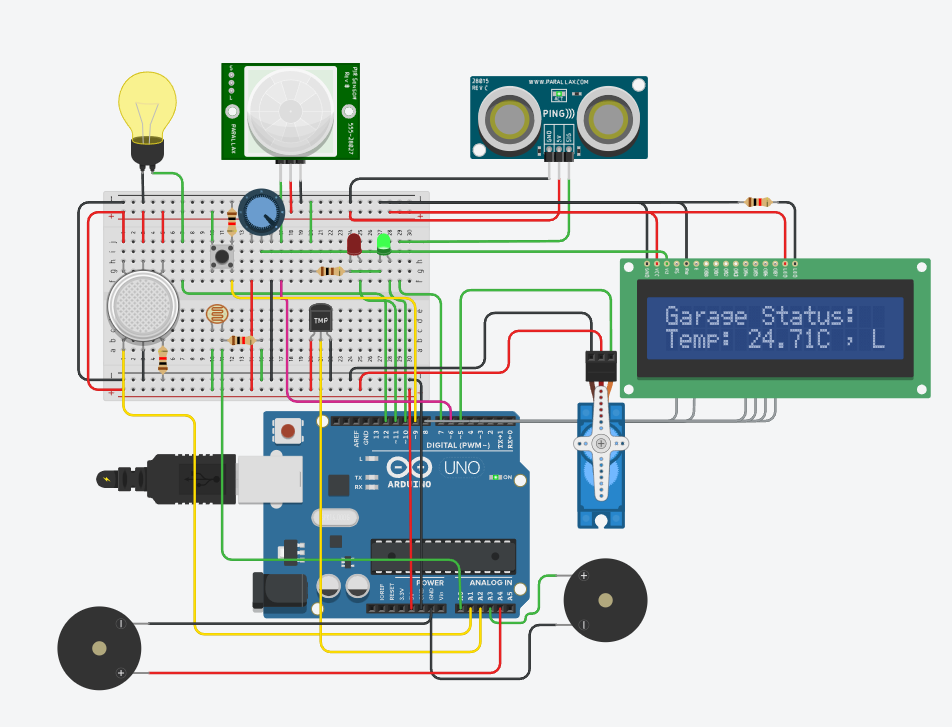
\includegraphics[width=\linewidth]{breadboard_view.png}
        \caption{Circuit design (Breadboard view)}
    \end{subfigure}
    \hfill
    \begin{subfigure}{0.45\textwidth}
        \centering
        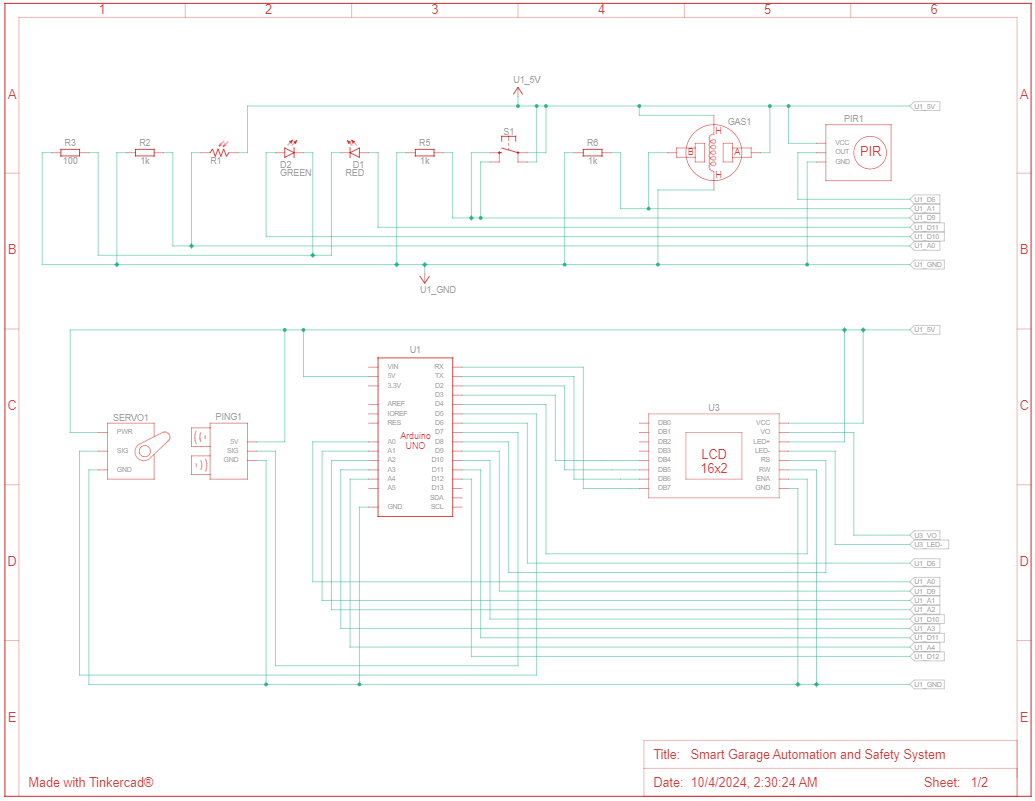
\includegraphics[width=\linewidth]{schematic_view.png}
        \caption{Circuit design (Schematic view)}
    \end{subfigure}
    \caption{Circuit Diagram of the Smart Garage Automation and Safety System}
    \label{fig:garage_circuit}
\end{figure}

\section{Code Snippet}
The following Arduino code controls the automation and safety features of the garage system:

\begin{lstlisting}[language=C++]
#include <Servo.h>
#include <LiquidCrystal.h> 

Servo servo;
LiquidCrystal lcd(8, 4, 3, 2, 1, 0);

int bulb = 12;
int red = 11;
int green = 10;
int smotar = 5;
int phsensor = A0;
int usdsensor = 7;
int pirsensor = 6;
int gassensor = A1;
int tempsensor = A2;
int button = 9;
int temPeizo = A3;
int gasPeizo = A4;

int lightFlag = 500;
int insideDistFlag = 100;
int gasFlag = 100;  
int tempFlag = 80;  

bool doorOpen = false;
bool carInside = false;
bool doorOpened = false;
bool gasAlert = false;
bool tempAlert = false;
bool alarmActive = false;

String scrollMsg = "";
int scrollIndex = 0;

void setup() {
  lcd.begin(16, 2);
  lcd.print("System Ready");
  delay(1000);
  lcd.clear();
  lcd.print("Created by");
  lcd.setCursor(1, 1);
  lcd.print("Pritom");
  delay(2000);
  lcd.clear();
  
  pinMode(phsensor, INPUT);
  pinMode(pirsensor, INPUT);
  pinMode(bulb, OUTPUT);
  pinMode(red, OUTPUT);
  pinMode(green, OUTPUT);
  pinMode(button, INPUT);
  pinMode(gassensor, INPUT);
  pinMode(tempsensor, INPUT);
  pinMode(gasPeizo, OUTPUT);
  pinMode(temPeizo, OUTPUT);
  servo.attach(smotar, 500, 2500);
  servo.write(0);
  delay(1000);
}

void handleDark() {
  int value = analogRead(phsensor);
  if(value > lightFlag) {
    digitalWrite(bulb, LOW); 
  } else {
    digitalWrite(bulb, HIGH); 
  }
}

void checkPresenceInside() {
  pinMode(usdsensor, OUTPUT);
  digitalWrite(usdsensor, LOW);
  delay(2);
  digitalWrite(usdsensor, HIGH);
  delay(10);
  digitalWrite(usdsensor, LOW);
  pinMode(usdsensor, INPUT);
  long duration = pulseIn(usdsensor, HIGH);
  long cm = (duration / 29) / 2;
  if(cm < insideDistFlag) {
    carInside = true;
    closeDoor();
  } else {
    carInside = false;
  }
}

void displayStatus() {
  if(carInside) {
    digitalWrite(red, LOW);
    digitalWrite(green, HIGH); 
  } else {
    digitalWrite(green, LOW);
    digitalWrite(red, HIGH);   
  }
}

void openDoor(int ms) {
  if(doorOpened) return;
  lcd.clear();
  lcd.print("Door Opening");
  delay(1000);
  servo.write(90);
  delay(2000 + ms);
  doorOpened = true;  
}

void closeDoor() {
  if(!doorOpened) return;
  lcd.clear();
  lcd.print("Door Closing");
  delay(1000);
  servo.write(0);
  delay(2000);
  doorOpened = false;  
}

void checkPir() {
  if(carInside) return;
  int value = digitalRead(pirsensor);
  if(value == HIGH)
    openDoor(0);
}

void checkButton() {
  if(!carInside) return;
  int value = digitalRead(button);
  if(value == HIGH) {
    openDoor(5000);
    closeDoor();
  }
}

void checkLeakage() {
  int gasValue = analogRead(gassensor); 

  if(gasValue > gasFlag) {
    gasAlert = true;
    lcd.clear();
    lcd.print("Gas Leak Alert");
    lcd.setCursor(0, 1);
    lcd.print("Gas: ");
    lcd.print(gasValue); 
    tone(gasPeizo, 2000); 
  } else {
    if (gasAlert) {
      gasAlert = false;
      noTone(gasPeizo); 
      lcd.clear();
      lcd.print("Gas Leak Cleared");
      delay(1000); 
    }
  }
}

void checkTemp() {
  int value = analogRead(tempsensor);
  float temp = value * 0.48828125 - 50; 

  if(temp > tempFlag) {
    tempAlert = true;
    lcd.clear();
    lcd.print("Temp Alert  ");
    lcd.setCursor(0, 1);
    lcd.print("Temp: ");
    lcd.print(temp);
    lcd.print("C"); 
    tone(temPeizo, 1000); 
  } else {
    if (tempAlert) {
      tempAlert = false;
      noTone(temPeizo); 
      lcd.clear();
      lcd.print("Temp Normal  ");
      delay(1000); 
    }
  }
}

void securityCheck() {
  if (!tempAlert && !gasAlert) {
    noTone(temPeizo);
    noTone(gasPeizo);
  } else if (tempAlert && gasAlert) {
    lcd.clear();
    lcd.print("Danger!!! Fire!!!");
    tone(temPeizo, 1000); 
    tone(gasPeizo, 2000); 
  }
}

void scrollStatus() {
  if (!tempAlert && !gasAlert) { 
    lcd.setCursor(0, 0);
    lcd.print("Garage Status:  ");

    lcd.setCursor(0, 1);
    lcd.print(scrollMsg.substring(scrollIndex, scrollIndex + 16)); 

    scrollIndex++;
    if(scrollIndex + 16 >= scrollMsg.length()) {
      scrollIndex = 0; 
    }

    delay(100); 
  }
}

void loop() {
  handleDark();
  checkPresenceInside();
  displayStatus();
  checkPir();
  checkButton();
  checkLeakage();
  checkTemp();
  securityCheck();
  if (!gasAlert && !tempAlert) {
    scrollMsg = "Temp: " + String(analogRead(tempsensor) * 0.48828125 - 50) + "C ";
    scrollMsg += (digitalRead(bulb) == HIGH ? ", Light On " : ", Light Off ");
    scrollMsg += (carInside ? ", Car Inside " : ", Car Outside ");
    scrollStatus(); 
  }
  delay(100); 
}
\end{lstlisting}

\section{System Output}
The system provides real-time feedback and automated actions based on sensor inputs, delivering essential features for the safety and automation of the garage.

One of the primary functions is the automated door control. The servo motor is responsible for opening and closing the garage door based on vehicle detection or manual input from the pushbutton. The ultrasonic sensor determines the vehicle's proximity to the garage, and the door opens or closes accordingly.

Additionally, the system is equipped with a gas sensor that monitors gas leakage within the garage. If a gas leak is detected, the system triggers an alert on the LCD and activates a buzzer for safety. Similarly, the system checks the ambient temperature, and if it exceeds the safety threshold, a high-temperature alert is activated.

For added convenience, manual control is available via the pushbutton, allowing the garage door to be opened or closed at will. LEDs (red and green) indicate whether the garage door is open or closed, providing a clear visual cue. The system also features motion detection using a PIR sensor, which can trigger an alarm or control the door based on activity within the garage area.

All sensor data is displayed on the 16x2 LCD screen, giving real-time feedback about the system's status. In the event of a gas leak or high temperature, the system will immediately provide a visible and audible alert to ensure prompt action.

\begin{figure}[H]
    \centering
    \begin{subfigure}{0.45\textwidth}
        \centering
        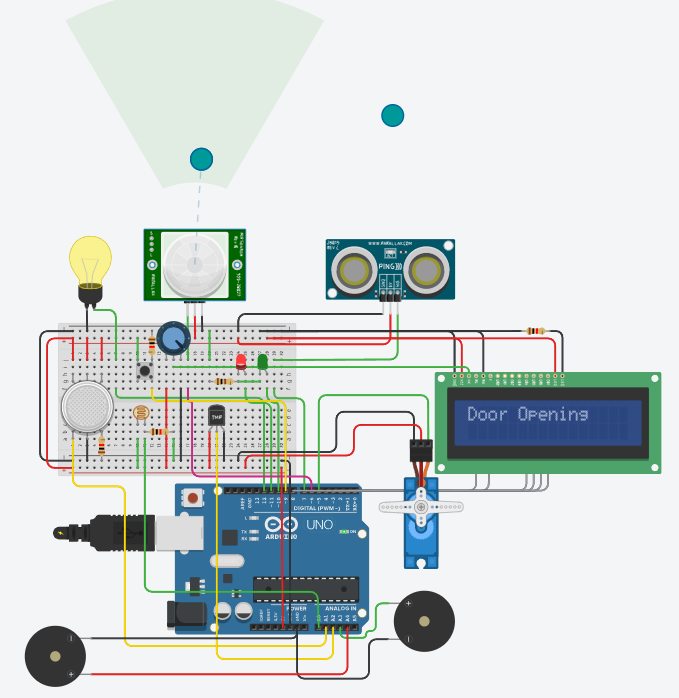
\includegraphics[width=\linewidth]{door_opening.png}
        \caption{Door Opening}
    \end{subfigure}
    \hfill
    \begin{subfigure}{0.45\textwidth}
        \centering
        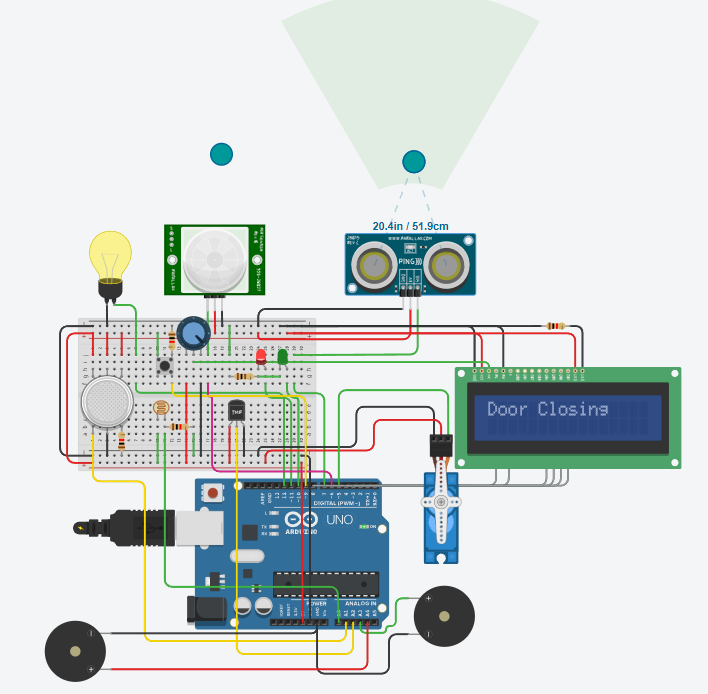
\includegraphics[width=\linewidth]{door_closing.png}
        \caption{Door Closing}
    \end{subfigure}
    
    \begin{subfigure}{0.45\textwidth}
        \centering
        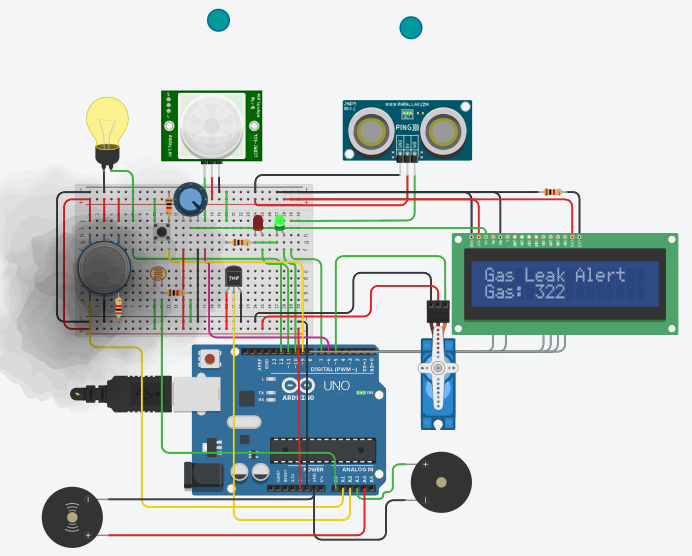
\includegraphics[width=\linewidth]{gas_alert.png}
        \caption{Gas Leak Alert}
    \end{subfigure}
    \hfill
    \begin{subfigure}{0.45\textwidth}
        \centering
        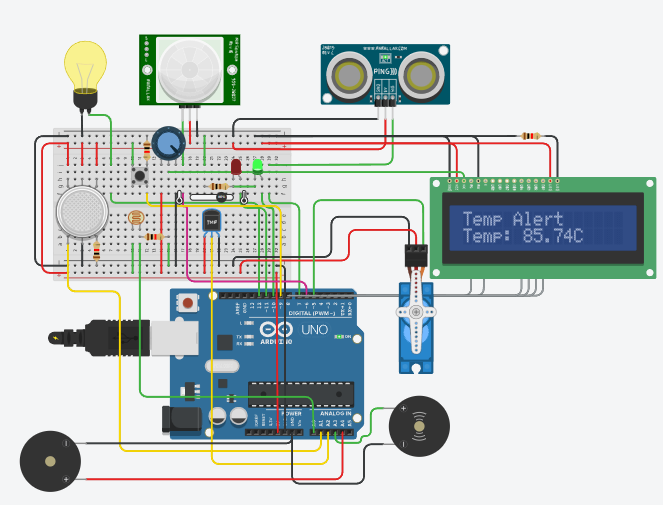
\includegraphics[width=\linewidth]{temp_alert.png}
        \caption{Temperature High Alert}
    \end{subfigure}
    \caption{System Output Showing Various Features of the Smart Garage}
    \label{fig:garage_output}
\end{figure}

\section{Conclusion}
The \textbf{Smart Garage Automation and Safety System} represents a significant advancement in home automation, combining convenience and safety in a single, user-friendly package. This system not only automates the operation of garage doors but also incorporates critical safety features, such as gas leak detection and temperature monitoring, which are crucial for maintaining a secure environment. By leveraging sensor technology and real-time feedback, this project offers a practical solution for modern living spaces, enhancing security and peace of mind for users. Future developments could include mobile app integration for remote monitoring and control, further extending the system's capabilities. As smart home technology continues to evolve, the Smart Garage Automation and Safety System stands out as a practical, innovative solution for enhancing everyday life.

\section{References}
\begin{enumerate}[label={[\arabic*]}]
    \item Arduino Uno R3 Documentation. Retrieved from \texttt{https://www.arduino.cc/en/Guide/ArduinoUno}
    \item Ultrasonic Sensor HC-SR04. Retrieved from \texttt{https://www.electronicwings.com/nodemcu/hc-sr04-ultrasonic-sensor-interfacing-with-nodemcu}
    \item PIR Sensor Overview. Retrieved from \texttt{https://learn.sparkfun.com/tutorials/pir-motion-sensor-hookup-guide/all}
    \item Servo Motor Control. Retrieved from \texttt{https://www.arduino.cc/en/Reference/Servo}
    \item LCD Display with Arduino. Retrieved from \texttt{https://www.arduino.cc/en/Tutorial/LiquidCrystal}
    \item Gas Sensor Operation. Retrieved from \texttt{https://www.electronicwings.com/nodemcu/gas-sensor-grove-interfacing-with-nodemcu}
\end{enumerate}

\end{document}
